\documentclass[10pt,twocolumn]{article}

\usepackage[margin=0.72in]{geometry}
\usepackage{amsmath,amssymb,amsthm,mathtools}
\usepackage{microtype}
\usepackage{times}
\usepackage[hidelinks]{hyperref}
\usepackage{enumitem}
\usepackage{graphicx}

\setlist{nosep,leftmargin=*}
\setlength{\columnsep}{0.22in}
\setlength{\parindent}{1em}
\setlength{\parskip}{0pt}
\emergencystretch=1em
\setcounter{dbltopnumber}{3}
\renewcommand{\dbltopfraction}{0.95}
\renewcommand{\dblfloatpagefraction}{0.85}
\renewcommand{\textfraction}{0.05}

\newtheorem{theorem}{Theorem}
\newtheorem{corollary}{Corollary}
\newtheorem{proposition}{Proposition}
\newtheorem{definition}{Definition}
\newtheorem{remark}{Remark}

\newcommand{\RR}{\mathbb{R}}
\newcommand{\CC}{\mathbb{C}}
\newcommand{\rank}{\operatorname{rank}}

\title{\vspace{-1.0em}Beyond Single-Exponential Self-Improvement:\
Takeoff Kernels, Response Modes, and Source Identification}
\author{Jonathan R. Landers}
\date{Working draft, July 2026}

\begin{document}
\maketitle
\vspace{-1.3em}

\begin{abstract}
A takeoff kernel records when eventual improvement is delivered; it need not
be exponential.  We use this general response object to recast a linearized
solver--verifier theory as a joint rank-one null: normalized solver, verifier,
and gap trajectories must share one discrete mode.  A finite-state extension
produces exponential response modes, but decomposing an observed kernel into
such modes is a source-separation problem, and response modes do not by
themselves identify mechanisms.  Synthetic studies confirm that rejecting
rank one is easier than recovering endpoints or modes.  In figure-derived
Phi-4 curves, one exact shared rate fails, while power-law relaxation often
matches or exceeds finite-modal forecasts and a shared phase-change model does
not win.  A resource-scaled reproduction closes the per-token gap without a
stable modal law.  Dense checkpoints further resolve one-optimizer-update
changes coupled to response length and accuracy, not a smooth capability
takeoff.  The evidence supports kernel-based response diagnosis and rejection
of a global shared-rate law, but not a discrete mode count, a universal local
exponential, or identified causal sources.
\end{abstract}

\section{Question and Scope}

A standard self-improvement loop generates candidate responses, evaluates or
filters them with a verifier, and trains the solver on the resulting signal
\cite{huang2025,song2025}.  Recent work by Sun et al.\ models the within-run
training trajectory through coupled solver and verifier uncertainties
\cite{sun2026}.  Its linearized theory predicts exponential convergence and an
intrinsic limit.  The present question is narrower than a general theory of
recursive intelligence: what finite response shape does this model predict,
and how can that prediction be tested or relaxed?

The answer begins with a distinction between two clocks.  The \emph{inner
clock} indexes optimization time or checkpoints within a training run.  The
\emph{outer clock} indexes complete generate--verify--retrain rounds.  The
theory analyzed below concerns the inner clock.  Applying the same kernel
language to the outer clock is possible, but the corresponding modes have a
different meaning and should be estimated separately.

The takeoff kernel itself makes no exponential assumption.  It is the sequence
of normalized checkpoint-to-checkpoint gains, and it can be concentrated,
long-tailed, signed, piecewise, or irregular.  Exponentials enter only when a
particular dynamical model is imposed.  An exponential curve approaching a
limit has a geometric residual, constant increment ratios, and rank-one Hankel
matrices.  For the coupled solver--verifier law, solver, verifier, and gap must
also share the same geometric mode.  This turns a visual curve-fitting claim
into a joint, falsifiable null without confusing the null with the general
kernel framework.

The theoretical development separates the response object from models of its
sources.  We first normalize increasing scores and decreasing uncertainties on
a common scale, then derive the rank-one restrictions implied by the standard
law.  A finite-dimensional hidden state gives one tractable subclass in which
active modes determine settling time and noiseless Hankel rank records modal
count.  Recovering those temporal components is already an inverse problem;
assigning them to solver learning, verifier drift, data refresh, or optimizer
state is a further source-identification problem.  A rank-one versus rank-two
construction isolates the basic point: identical endpoints need not imply
similar finite takeoff.

The empirical half asks what can actually be learned from short, noisy
trajectories.  Synthetic studies first separate rejection of rank one from the
harder tasks of estimating the asymptote and recovering individual modes.  We
then examine vector-extracted Phi-4 trajectories from Sun et al., run a
resource-scaled fresh-seed reproduction, compare global modal, time-local, and
nonmodal forecasts, and repeat one seed with quarter-epoch measurements through
epoch four.  The published curves are inconsistent with one exact shared rate,
but neither they nor the reproduction identify a stable replacement mode count
or local exponential.  The intended outcome is therefore a sharper inverse
problem and measurement protocol, not a claim that hidden mechanisms have been
recovered.

\section{Response Normalization}

Let $Y_n$ be a scalar observable measured at equally spaced checkpoints and
suppose $Y_n\to Y_\infty$ with $Y_0\ne Y_\infty$.  The observable may be an
increasing performance score or a decreasing uncertainty.  The following
normalization treats both cases identically.

\begin{definition}[Residual, profile, and takeoff kernel]
Define
\begin{equation}\label{eq:normalization}
 e_n=\frac{Y_n-Y_\infty}{Y_0-Y_\infty},
 \qquad
 F_n=1-e_n,
\end{equation}
and, for $n\geq1$,
\begin{equation}\label{eq:kernel}
 \kappa_n=F_n-F_{n-1}=e_{n-1}-e_n.
\end{equation}
The sequence $e_n$ is the normalized residual distance to the limit, $F_n$ is
the cumulative realized response, and $\kappa_n$ is the response delivered at
checkpoint $n$.
\end{definition}

By telescoping,
\begin{equation}\label{eq:telescope}
 \sum_{j=1}^{N}\kappa_j=F_N=1-e_N.
\end{equation}
Hence $\sum_{j\geq1}\kappa_j=1$ whenever $e_n\to0$.  If $F_n$ is monotone,
the kernel is nonnegative and can be read as a distribution of improvement
over checkpoints.  Negative entries instead mark regression, overshoot, or
ringing.  With this common scale in place, a single exponential becomes an
exact algebraic hypothesis rather than a qualitative curve shape.

\begin{remark}[The kernel precedes its parameterization]
Equations~\eqref{eq:normalization}--\eqref{eq:kernel} define a kernel for any
convergent observed trajectory once an endpoint and clock are fixed.  They do
not require linearity, smoothness, or an exponential mixture.  Finite modal,
power-law, phase-changing, and nonparametric laws are competing descriptions
of the kernel, not competing definitions of it.  Consequently, the kernel
formalism alone is descriptive; empirical content comes from restrictions that
forecast untouched checkpoints and replicate across seeds.
\end{remark}

\section{The Standard Law Is Rank One}

The first result identifies exactly what a single exponential asserts about
the finite response.

\begin{theorem}[Single-mode equivalence]\label{thm:single-mode}
Let $e_0=1$, let $e_n\to0$, and define $\kappa_n=e_{n-1}-e_n$ for $n\geq1$.
For any $\lambda\in\CC$ with $|\lambda|<1$, the following are equivalent:
\begin{align}
 e_n&=\lambda^n &&(n\geq0), \label{eq:geometric-residual}\\
 \kappa_n&=(1-\lambda)\lambda^{n-1} &&(n\geq1).
 \label{eq:geometric-kernel}
\end{align}
When the response is real and monotone, $\lambda\in[0,1)$.  Moreover, wherever
the ratios are defined,
\begin{equation}\label{eq:ratio-test}
 \frac{\kappa_{n+1}}{\kappa_n}=\lambda,
\end{equation}
and every adjacent second-order Hankel minor vanishes:
\begin{equation}\label{eq:hankel-test}
 \kappa_{n+1}\kappa_{n-1}-\kappa_n^2=0.
\end{equation}
\end{theorem}

\begin{proof}
If $e_n=\lambda^n$, then
\[
 \kappa_n=e_{n-1}-e_n
 =\lambda^{n-1}-\lambda^n
 =(1-\lambda)\lambda^{n-1}.
\]
Conversely, if \eqref{eq:geometric-kernel} holds, telescoping gives
\[
 F_n=\sum_{j=1}^{n}(1-\lambda)\lambda^{j-1}=1-\lambda^n.
\]
Since $e_n=1-F_n$, equation \eqref{eq:geometric-residual} follows.  Equations
\eqref{eq:ratio-test} and \eqref{eq:hankel-test} follow by direct substitution.
If the real response is monotone, then $0\leq e_{n+1}\leq e_n$ and therefore
$\lambda\in[0,1)$.
\end{proof}

The theorem replaces a visual statement about curve shape by local algebraic
restrictions.  A high in-sample coefficient of determination for an
exponential fit does not by itself test those restrictions, especially when
the asymptote is also estimated.

\subsection{Application to solver--verifier dynamics}

Sun et al.\ define solver uncertainty $U_s(t)$, verifier uncertainty $U_v(t)$,
and gap
\begin{equation}\label{eq:gap}
 G(t)=U_s(t)-U_v(t).
\end{equation}
Their phenomenological dynamics are
\begin{equation}\label{eq:sun-dynamics}
 \frac{dU_s}{dt}=-\alpha E(t),
 \qquad
 \frac{dU_v}{dt}=-\beta E(t),
 \qquad \alpha>\beta\geq0,
\end{equation}
where $E(t)=f(G(t))$.  Around an initial state they use the affine
approximation
\begin{equation}\label{eq:linear-potential}
 E(t)\approx kG(t)-b.
\end{equation}
Writing $G_\infty=b/k$ and $\gamma=k(\alpha-\beta)>0$, their solution has the
form
\begin{align}
 G(t)-G_\infty&=C_Ge^{-\gamma t},\label{eq:gap-solution}\\
 U_s(t)-U_{s,\infty}&=C_se^{-\gamma t},\label{eq:solver-solution}\\
 U_v(t)-U_{v,\infty}&=C_ve^{-\gamma t},\label{eq:verifier-solution}
\end{align}
for constants determined by the initial condition.

\begin{corollary}[Kernel form of the solver--verifier law]
\label{cor:sun-kernel}
Sample \eqref{eq:gap-solution}--\eqref{eq:verifier-solution} at times
$t_n=n\Delta$ with $\Delta>0$.  For every nonconstant observable
$X\in\{G,U_s,U_v\}$, its normalized residual and takeoff kernel are
\begin{equation}\label{eq:sun-kernel}
 e_n^{(X)}=\lambda^n,
 \qquad
 \kappa_n^{(X)}=(1-\lambda)\lambda^{n-1},
 \qquad
 \lambda=e^{-k(\alpha-\beta)\Delta}.
\end{equation}
Thus the three normalized trajectories share one mode, and each exact kernel
Hankel matrix has rank one.
\end{corollary}

\begin{proof}
For a nonconstant $X$, equations
\eqref{eq:gap-solution}--\eqref{eq:verifier-solution} give
\[
 \frac{X(t_n)-X_\infty}{X(0)-X_\infty}
 =e^{-\gamma n\Delta}=\lambda^n.
\]
Apply Theorem~\ref{thm:single-mode}.  The sequence
$\kappa_n=(1-\lambda)\lambda^{n-1}$ is an outer product on any Hankel grid, so
its nonzero Hankel matrix has rank one.
\end{proof}

\begin{corollary}[Joint empirical null]\label{cor:joint-null}
Under \eqref{eq:sun-dynamics}--\eqref{eq:linear-potential}, equally spaced
observations obey all of the following restrictions:
\begin{enumerate}
 \item $e_n^{(s)}=e_n^{(v)}=e_n^{(G)}$ whenever the three normalizations exist;
 \item each kernel has the same constant ratio $\lambda$;
 \item every second-order kernel Hankel minor vanishes;
 \item if $\beta>0$, then
 \[
  \frac{U_s(t)-U_{s,\infty}}{U_v(t)-U_{v,\infty}}
  =\frac{\alpha}{\beta}
 \]
 throughout the nonstationary trajectory.
\end{enumerate}
\end{corollary}

\begin{proof}
The first three statements follow from Corollary~\ref{cor:sun-kernel}.  For the
fourth, integrating \eqref{eq:sun-dynamics} from $t$ to infinity gives
\begin{align*}
 U_s(t)-U_{s,\infty}
 &=\alpha\int_t^\infty E(\tau)\,d\tau,\\
 U_v(t)-U_{v,\infty}
 &=\beta\int_t^\infty E(\tau)\,d\tau.
\end{align*}
Taking the ratio proves the claim.
\end{proof}

Corollary~\ref{cor:joint-null} is the first result to test empirically.  It is
strictly sharper than fitting one exponential to each series independently:
it tests whether all observables arise from the same one-dimensional active
response.

\section{Finite-Dimensional Modal Generalization}

The rank-one null can be relaxed without abandoning a tractable response law,
but this is a model class for the observed response, not a definition of the
kernel and not yet a claim about its physical sources.  Let
Let $x_n\in\CC^d$ be a hidden state centered at its limiting value and suppose
that, over the observation window, it evolves linearly:
\begin{equation}\label{eq:state-space}
 x_{n+1}=Ax_n.
\end{equation}
Let the centered scalar observable be
\begin{equation}\label{eq:observation}
 y_n=Y_n-Y_\infty=c^*x_n.
\end{equation}

\begin{theorem}[Modal takeoff representation]\label{thm:modal}
Assume $A$ is diagonalizable over $\CC$.  Let
$\theta_1,\ldots,\theta_R$ be the distinct eigenvalues that are active for the
initial state $x_0$ and observation vector $c$, and assume
$|\theta_j|<1$.  Then there are nonzero modal amplitudes
$a_1,\ldots,a_R$ such that
\begin{equation}\label{eq:modal-observable}
 y_n=\sum_{j=1}^{R}a_j\theta_j^n.
\end{equation}
If $y_0=\sum_j a_j\ne0$, the normalized residual and takeoff kernel are
\begin{align}
 e_n&=\frac{\sum_{j=1}^{R}a_j\theta_j^n}
 {\sum_{j=1}^{R}a_j},\label{eq:modal-residual}\\
 \kappa_n&=\frac{\sum_{j=1}^{R}a_j(1-\theta_j)
 \theta_j^{n-1}}{\sum_{j=1}^{R}a_j}.
 \label{eq:modal-kernel}
\end{align}
For real $A,c,x_0$, nonreal modes and amplitudes occur in conjugate pairs, so
$e_n$ and $\kappa_n$ remain real.
\end{theorem}

\begin{proof}
Diagonalizability gives right eigenvectors $v_j$ and spectral projectors
$P_j$ such that
\[
 A^n=\sum_j\theta_j^nP_j.
\]
Substituting this expansion into \eqref{eq:observation} gives
\[
 y_n=c^*A^nx_0
 =\sum_j(c^*P_jx_0)\theta_j^n.
\]
Discard terms with zero coefficient and combine repeated eigenvalues.  This
produces \eqref{eq:modal-observable} with the distinct active modes.  Since
$y_0=\sum_j a_j$, division by $y_0$ gives
\eqref{eq:modal-residual}.  Taking the difference $e_{n-1}-e_n$ gives
\eqref{eq:modal-kernel}.  For real data, the real canonical form pairs every
nonreal eigenvalue with its complex conjugate, and the corresponding terms sum
to a real sequence.
\end{proof}

\begin{remark}[What the standard model suppresses]
After centering on its trajectory-specific limit, the linearized
solver--verifier system has matrix
\begin{equation}\label{eq:sun-matrix}
 B=-k
 \begin{pmatrix}
  \alpha&-\alpha\\
  \beta&-\beta
 \end{pmatrix}.
\end{equation}
Its eigenvalues are $0$ and $-k(\alpha-\beta)$.  The zero direction parametrizes
the continuum of stationary endpoints and vanishes after centering on the
endpoint selected by the initial condition.  Only the decaying direction is
active, which explains rank one.  A general stable two-state Jacobian has two
decaying eigenvalues; sampling it at interval $\Delta$ yields modes
$\theta_j=e^{\mu_j\Delta}$ and hence a rank-at-most-two modal kernel.
\end{remark}

Theorem~\ref{thm:modal} does not identify mechanisms from a curve.  It
identifies response modes.  Assigning a recovered fast or slow mode to solver
learning, verifier drift, data refresh, or optimizer state requires additional
measurements or interventions.

\subsection{Response modes versus latent sources}

The distinction can be written as a small source-separation problem.  Suppose
the centered measured observables are
\begin{equation}\label{eq:source-mixing}
 \mathbf y_n=C\mathbf z_n,\qquad \mathbf z_{n+1}=A\mathbf z_n,
\end{equation}
where the coordinates of $\mathbf z_n$ are latent response channels and $C$
is an unknown observation map.  Diagonalizing $A$ gives temporal response modes
in each measured curve, but it does not determine the columns of $C$ or attach
them to named training mechanisms.  Different latent systems can therefore
produce the same observed kernel.

In the solver--verifier data, this ambiguity is particularly sharp.  The gap
is derived, $G=U_s-U_v$, so the three plotted curves are not three independent
sensors.  A fitted second mode is evidence for a second effective timescale in
the response model; it is not, by itself, evidence for a second causal source.
Source separation requires additional independent observables, repeated
conditions with different mixing weights, or interventions that selectively
perturb a channel.  The empirical analyses below therefore separate response
diagnosis from mechanistic attribution.

\section{Modal Radius and Settling}

The modal representation tells us what components are present.  We next ask
what those components imply for the time required to approach the endpoint.

\begin{definition}[Settling time]
For $\epsilon>0$, define
\begin{equation}\label{eq:settling-definition}
 T_\epsilon
 =
 \min\{N\geq0: |e_n|\leq\epsilon\text{ for every }n\geq N\}.
\end{equation}
\end{definition}

The modal radius must refer to modes active in the measured observable, not to
every eigenvalue of a latent transition matrix.

\begin{theorem}[Modal radius controls settling]\label{thm:settling}
Under the hypotheses of Theorem~\ref{thm:modal}, write
$d_j=a_j/\sum_\ell a_\ell$ and let
\begin{equation}\label{eq:modal-radius}
 \lambda_\star=\max_{1\leq j\leq R}|\theta_j|,
 \qquad 0<\lambda_\star<1.
\end{equation}
There are constants $0<c\leq C<\infty$ such that, for every $n\geq0$,
\begin{align}
 |e_n|&\leq C\lambda_\star^n,\label{eq:settling-upper}\\
 \max_{0\leq \ell<R}|e_{n+\ell}|
 &\geq c\lambda_\star^n.\label{eq:block-lower}
\end{align}
Consequently, for all sufficiently small $\epsilon>0$,
\begin{equation}\label{eq:settling-bounds}
 \frac{\log(c/\epsilon)}{-\log\lambda_\star}
 \leq T_\epsilon
 \leq
 \left\lceil
 \frac{\log(C/\epsilon)}{-\log\lambda_\star}
 \right\rceil,
\end{equation}
and hence
\begin{equation}\label{eq:settling-asymptotic}
 \lim_{\epsilon\downarrow0}
 \frac{T_\epsilon}{\log(1/\epsilon)}
 =
 \frac{1}{-\log\lambda_\star}.
\end{equation}
\end{theorem}

\begin{proof}
Equation~\eqref{eq:modal-residual} gives
\[
 |e_n|
 \leq \sum_{j=1}^{R}|d_j||\theta_j|^n
 \leq
 \left(\sum_{j=1}^{R}|d_j|\right)\lambda_\star^n,
\]
so \eqref{eq:settling-upper} holds with
$C=\sum_j|d_j|$.

For the lower bound, let $V$ be the square Vandermonde matrix
\[
 V_{\ell j}=\theta_j^\ell,
 \qquad 0\leq\ell<R,\quad 1\leq j\leq R.
\]
The modes are distinct, so $V$ is invertible.  Define
$q_n=(d_1\theta_1^n,\ldots,d_R\theta_R^n)^\top$.  The block of $R$
successive residuals is
\[
 (e_n,\ldots,e_{n+R-1})^\top=Vq_n.
\]
Let $\sigma_{\min}(V)>0$ be the smallest singular value.  Since at least one
active coefficient $d_j$ has $|\theta_j|=\lambda_\star$,
\[
 \max_{0\leq\ell<R}|e_{n+\ell}|
 \geq
 \frac{\sigma_{\min}(V)}{\sqrt R}\|q_n\|_2
 \geq c\lambda_\star^n
\]
for a fixed $c>0$.  This proves \eqref{eq:block-lower}.

The upper bound in \eqref{eq:settling-bounds} follows because every $m\geq N$
obeys $|e_m|\leq C\lambda_\star^N$.  If the trajectory has settled by
$T_\epsilon$, every member of its next length-$R$ block is at most $\epsilon$,
so \eqref{eq:block-lower} gives
$c\lambda_\star^{T_\epsilon}\leq\epsilon$, which is the lower bound.
Dividing by $\log(1/\epsilon)$ and sending $\epsilon\downarrow0$ proves
\eqref{eq:settling-asymptotic}.
\end{proof}

\begin{remark}[Cancellation and visible modes]\label{rem:cancellation}
An eigenvalue of $A$ is absent when its coefficient
$a_j=c^*P_jx_0$ vanishes.  Such a mode is unexcited by the initial condition,
unobserved by the measurement, or both; it cannot be inferred from that scalar
trajectory.  Equal-radius active modes can also cancel at isolated
checkpoints.  The block lower bound in Theorem~\ref{thm:settling} shows why
those cancellations do not change the asymptotic settling exponent.
\end{remark}

\begin{remark}[Shape classes]
If $\theta_j\in[0,1)$ and $d_j\geq0$ for every $j$, then
\[
 \kappa_n=\sum_j d_j(1-\theta_j)\theta_j^{n-1}\geq0,
\]
so the response is monotone.  Negative real modes can alternate, while
nonreal conjugate pairs produce damped ringing.  These are implications of the
fitted response modes, not yet causal labels for training mechanisms.
\end{remark}

\begin{remark}[Jordan blocks and repeated modes]\label{rem:jordan}
If $A$ is not diagonalizable, a Jordan block replaces a pure exponential by
$p_j(n)\theta_j^n$, where $p_j$ is a polynomial whose degree is smaller than
the block size.  For largest active block size $m$,
\[
 |e_n|\leq Cn^{m-1}\lambda_\star^n.
\]
The leading settling scale remains $\log(1/\epsilon)/(-\log\lambda_\star)$,
with at most an additional order-$\log\log(1/\epsilon)$ correction.  Thus a
repeated mode is not correctly represented by simply listing the same
eigenvalue several times in Theorem~\ref{thm:modal}.
\end{remark}

\begin{remark}[Algebraic tails are outside the finite-modal model]
If $e_n\sim cn^{-p}$ with $c\ne0$ and $p>0$, then
$|e_n|^{1/n}\to1$ and $T_\epsilon$ grows on the order of
$\epsilon^{-1/p}$.  No finite sum of stable polynomial--exponential modes can
equal such a tail eventually, because every such sum has root-decay rate
strictly below one.  An observed algebraic tail therefore points to
time-varying, infinite-dimensional, or broad-spectrum dynamics rather than a
larger but finite stable modal order.

For completely monotone residuals, a broad spectrum can be represented as a
positive mixture of exponentials,
\begin{equation}\label{eq:diffuse-spectrum}
 e(t)=\int_0^\infty e^{-\lambda t}\,d\mu(\lambda),
\end{equation}
with a finite-modal response corresponding to an atomic measure $\mu$.  This
representation is a useful comparison class, not a universal representation
of arbitrary signed or phase-changing kernels.  A power-law forecast can thus
be a compact description of many timescales without identifying a finite list
of modes.
\end{remark}

\section{Hankel Rank and Exact Modal Recovery}

Settling is the forward consequence of the active modes.  The corresponding
inverse question is whether those modes can be counted and recovered from the
observed response.

Write the modal kernel from \eqref{eq:modal-kernel} as
\begin{equation}\label{eq:kernel-modal-sum}
 \kappa_n=\sum_{j=1}^{R}b_j\theta_j^{n-1},
 \qquad
 b_j=d_j(1-\theta_j).
\end{equation}
Because $|\theta_j|<1$, every active $d_j$ gives a nonzero $b_j$.

\begin{theorem}[Hankel rank equals active modal count]\label{thm:hankel-rank}
Let $\theta_1,\ldots,\theta_R$ be distinct and let $b_j\ne0$.  For $m\geq R$,
form the square kernel Hankel matrix
\begin{equation}\label{eq:hankel-matrix}
 H_m=(\kappa_{i+j+1})_{i,j=0}^{m-1}.
\end{equation}
Then
\begin{equation}\label{eq:hankel-rank}
 \rank H_m=R.
\end{equation}
In particular, the leading $R\times R$ determinant is
\begin{equation}\label{eq:hankel-determinant}
 \det H_R
 =
 \left(\prod_{j=1}^{R}b_j\right)
 \left(\prod_{1\leq p<q\leq R}
 (\theta_q-\theta_p)^2\right)
 \ne0.
\end{equation}
\end{theorem}

\begin{proof}
Let $V_m$ be the $m\times R$ Vandermonde matrix
$(V_m)_{ij}=\theta_j^i$ for $0\leq i<m$.  Equation
\eqref{eq:kernel-modal-sum} gives the factorization
\begin{equation}\label{eq:hankel-factorization}
 H_m=V_m\operatorname{diag}(b_1,\ldots,b_R)V_m^\top.
\end{equation}
Thus $\rank H_m\leq R$.  When $m=R$, the Vandermonde determinant is
$\det V_R=\prod_{p<q}(\theta_q-\theta_p)$, so
\eqref{eq:hankel-determinant} follows and $H_R$ is nonsingular.  For $m>R$,
$H_R$ is a nonsingular principal submatrix of $H_m$, giving
$\rank H_m\geq R$.  Hence equality holds.
\end{proof}

\begin{corollary}[Noiseless matrix-pencil recovery]\label{cor:matrix-pencil}
Define
\begin{equation}\label{eq:hankel-pencil}
 H_0=(\kappa_{i+j+1})_{i,j=0}^{R-1},
 \qquad
 H_1=(\kappa_{i+j+2})_{i,j=0}^{R-1}.
\end{equation}
Then the generalized eigenvalues of the pencil $(H_1,H_0)$ are precisely
$\theta_1,\ldots,\theta_R$:
\begin{equation}\label{eq:pencil-determinant}
 \det(H_1-zH_0)
 =
 \det(V_R)^2
 \left(\prod_{j=1}^{R}b_j\right)
 \prod_{j=1}^{R}(\theta_j-z).
\end{equation}
Thus $2R$ consecutive kernel values suffice for exact modal recovery in the
nondegenerate noiseless model.
\end{corollary}

\begin{proof}
With $\Theta=\operatorname{diag}(\theta_1,\ldots,\theta_R)$ and
$D=\operatorname{diag}(b_1,\ldots,b_R)$, the two matrices factor as
\[
 H_0=V_RDV_R^\top,
 \qquad
 H_1=V_RD\Theta V_R^\top.
\]
Taking the determinant of
$V_RD(\Theta-zI)V_R^\top$ proves \eqref{eq:pencil-determinant}.
\end{proof}

Exact rank is not a literal noisy-data estimator: an arbitrarily small generic
perturbation makes a finite Hankel matrix full rank.  The empirical analogue
must therefore use a singular-value spectrum, regularization, bootstrap
stability, and held-out prediction.  Theorem~\ref{thm:hankel-rank} supplies the
population target for that procedure.

\section{Same Endpoints, Different Takeoff}

The recovery results make modal order observable in principle.  The following
construction shows why that order matters even when the usual endpoint
comparison cannot distinguish two trajectories.

\begin{corollary}[Endpoint separation]\label{cor:endpoint-separation}
Fix $Y_0\ne Y_\infty$, $0<a<b<1$, and $w\in(0,1)$.  Define
\begin{align}
 Y_n^{(1)}
 &=Y_\infty+(Y_0-Y_\infty)a^n,\label{eq:endpoint-one}\\
 Y_n^{(2)}
 &=Y_\infty+(Y_0-Y_\infty)
 \bigl(wa^n+(1-w)b^n\bigr).\label{eq:endpoint-two}
\end{align}
The trajectories have the same initial value, limit, and total normalized
kernel mass.  The first has Hankel rank one and modal radius $a$; the second
has Hankel rank two and modal radius $b$.  Their kernels are
\begin{align}
 \kappa_n^{(1)}
 &=(1-a)a^{n-1},\label{eq:endpoint-kernel-one}\\
 \kappa_n^{(2)}
 &=w(1-a)a^{n-1}
 +(1-w)(1-b)b^{n-1}.\label{eq:endpoint-kernel-two}
\end{align}
Moreover, for $0<\epsilon<1-w$,
\begin{equation}\label{eq:endpoint-settling}
 T_\epsilon^{(1)}
 =
 \left\lceil\frac{\log\epsilon}{\log a}\right\rceil,
 \qquad
 T_\epsilon^{(2)}
 \geq
 \frac{\log((1-w)/\epsilon)}{-\log b}.
\end{equation}
For fixed $a,w,\epsilon$, the second settling time becomes arbitrarily large
as $b\uparrow1$, although the endpoints remain unchanged.
\end{corollary}

\begin{proof}
Both normalized residuals equal one at $n=0$ and converge to zero.  Taking
successive differences gives
\eqref{eq:endpoint-kernel-one}--\eqref{eq:endpoint-kernel-two}; both kernels
are nonnegative and telescope to total mass one.  The rank statements follow
from Theorem~\ref{thm:hankel-rank}.  The first settling formula follows from
$a^n\leq\epsilon$.  Since the second residual satisfies
$e_n^{(2)}\geq(1-w)b^n$, settling requires
$(1-w)b^n\leq\epsilon$, which gives the stated lower bound.
\end{proof}

Corollary~\ref{cor:endpoint-separation} is the first synthetic experiment.  It
shows exactly what endpoint or final-gain comparisons omit: the slow mode can
carry modest weight while controlling the late response.

\begin{figure*}[t]
\centering
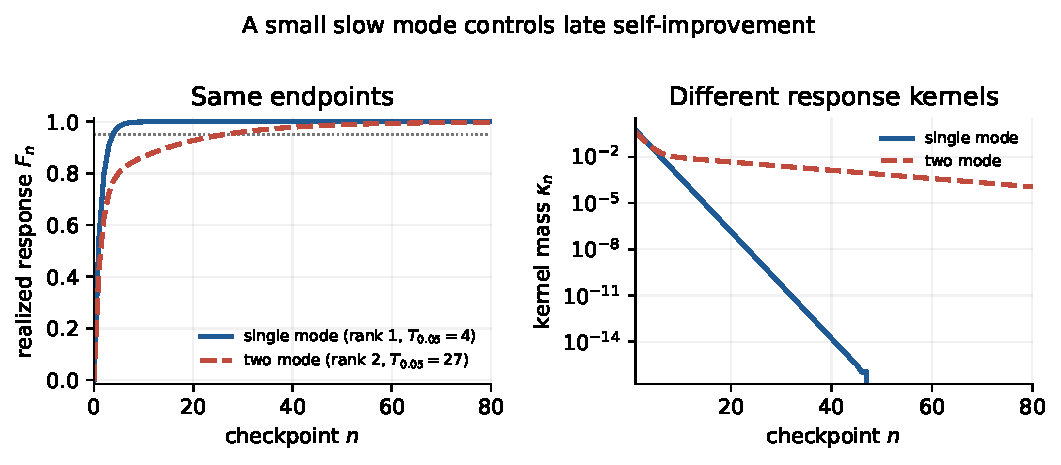
\includegraphics[width=0.94\textwidth]{figures/fig1_endpoint_separation.pdf}
\caption{\textbf{Same endpoints, different response kernels.}
The rank-one trajectory uses $a=0.45$.  The rank-two trajectory assigns weight
$w=0.75$ to that fast mode and weight $0.25$ to a slow mode $b=0.94$.  Both
profiles begin at zero, converge to one, and have total kernel mass one.
Nevertheless, their exact Hankel ranks are one and two, and their
$\epsilon=0.05$ settling times are $4$ and $27$ checkpoints.  The slow mode is
lightly weighted in the early response but controls the tail.}
\label{fig:endpoint-separation}
\end{figure*}

\section{Synthetic Detectability}

Exact Hankel rank is discontinuous under noise, so Theorem
\ref{thm:hankel-rank} does not by itself determine how many checkpoints an
experiment needs.  We estimate that requirement for the construction in
Figure~\ref{fig:endpoint-separation}.  The null residual is
\begin{equation}\label{eq:power-null}
 e_n^{(0)}=0.45^n,
\end{equation}
and the rank-two alternative is
\begin{equation}\label{eq:power-alternative}
 e_n^{(1)}=0.75(0.45)^n+0.25(0.94)^n.
\end{equation}
At each checkpoint after $n=0$, we add independent Gaussian noise with
standard deviation $\sigma$ on the normalized residual scale.  The baseline
$e_0=1$ and the limiting endpoint are treated as known in this first power
study.

For $N$ observed checkpoints, use the common square size
$m=\lfloor N/2\rfloor$, the largest size supported by the corresponding
length-$(N-1)$ kernel, and form an $m\times m$ Hankel matrix from either $e_n$
or $\kappa_n=e_{n-1}-e_n$.  The test statistic is the singular-value ratio
\begin{equation}\label{eq:power-statistic}
 S=\frac{s_2(H)}{s_1(H)}.
\end{equation}
An independent set of $2{,}000$ rank-one simulations calibrates the upper
five-percent threshold.  A second null set checks the false-positive rate, and
$2{,}000$ rank-two simulations estimate power.  The largest absolute
false-positive calibration error across nonzero-noise conditions is $0.014$.

\begin{figure*}[t]
\centering
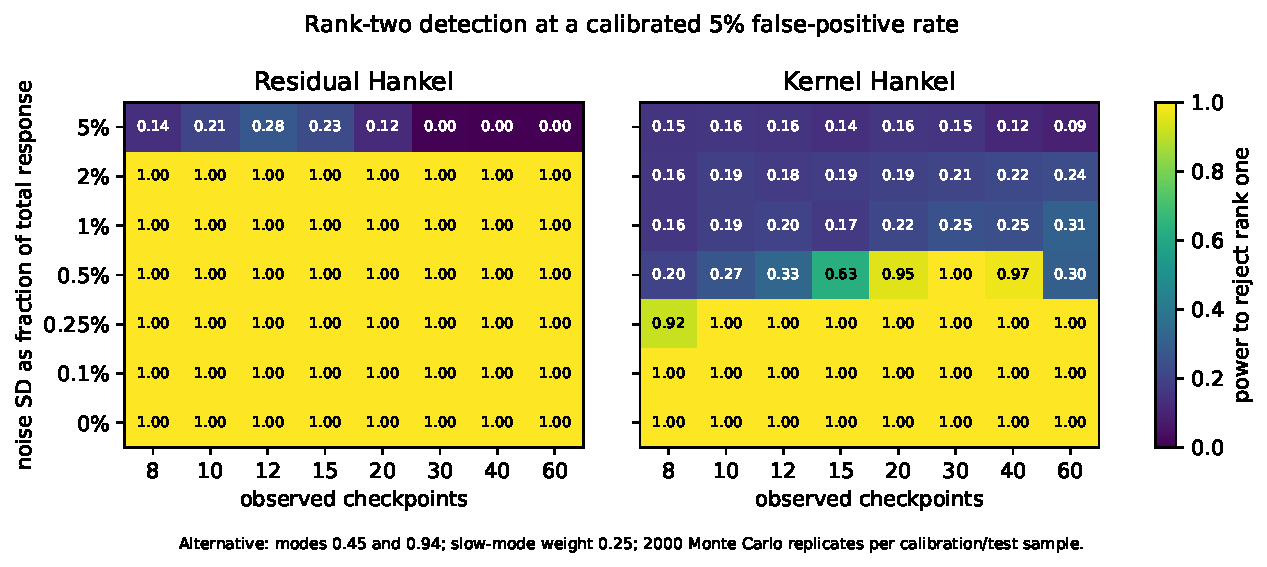
\includegraphics[width=0.96\textwidth]{figures/fig2_modal_power.pdf}
\caption{\textbf{Power to detect the slow second mode.}
Each cell reports the probability of rejecting rank one using the calibrated
singular-value-ratio statistic \eqref{eq:power-statistic}.  With the endpoint
known, the residual Hankel detects the rank-two alternative with at least
$0.8$ power from eight checkpoints through $\sigma=0.02$.  Kernel Hankels are
more demanding: eight checkpoints suffice through $\sigma=0.0025$, while
twenty are required at $\sigma=0.005$; no tested count reaches $0.8$ power at
$\sigma\geq0.01$.  Enlarging an unregularized square Hankel can eventually add
more noise-only tail than signal, so power need not be monotone in the plotted
checkpoint count.}
\label{fig:modal-power}
\end{figure*}

The gap between the panels has a direct modal explanation.  In the residual,
the slow-mode amplitude is $d_{\rm slow}=0.25$.  In the kernel it becomes
\[
 b_{\rm slow}
 =
 d_{\rm slow}(1-\theta_{\rm slow})
 =
 0.25(1-0.94)=0.015.
\]
Relative to the fast mode, differencing attenuates the slow component by the
additional factor
\begin{equation}\label{eq:slow-attenuation}
 \frac{1-\theta_{\rm slow}}{1-\theta_{\rm fast}}
 =
 \frac{0.06}{0.55}
 \approx0.109,
\end{equation}
while independent observation noise acquires a differenced standard deviation
of approximately $\sqrt2\,\sigma$.  Residual Hankels are therefore preferable
for detecting modal order when the asymptote is trustworthy; kernels remain
the natural object for interpreting when improvement arrives.

These numbers are design guidance for this alternative, not a universal
sample-complexity theorem.  They are optimistic about the residual because
$Y_\infty$ is known.  An asymptote error introduces a nearly constant residual
component and can mimic an additional mode.  The next sensitivity analysis
therefore profiles over $Y_\infty$ and compares held-out modal fits.  Varying
slow-mode weight and separation, and comparing regularized or windowed
Hankels, remain subsequent robustness checks.

\section{Unknown Asymptote and Held-Out Forecasting}

We next remove the known-endpoint advantage.  On a training prefix, we fit
the nested models
\begin{align}
 Y_n^{[1]}&=Y_\infty+c\lambda^n,\label{eq:unknown-rank-one}\\
 Y_n^{[2]}&=Y_\infty+c_1\theta_1^n+c_2\theta_2^n,\label{eq:unknown-rank-two}
\end{align}
with $c,c_1,c_2\geq0$ and $Y_\infty\in[-0.25,0.25]$.  For each candidate
mode tuple on a fixed grid, the endpoint and amplitudes are obtained by linear
least squares; the grid search then selects the smallest training error.  The
last quarter of the checkpoints, with at least three held out, is used only for
forecasting.  Model preference is measured by
\begin{equation}\label{eq:heldout-score}
 D=\log\frac{\operatorname{MSE}_{\rm holdout}^{[1]}}
                 {\operatorname{MSE}_{\rm holdout}^{[2]}}.
\end{equation}
For every noise level and checkpoint count, an independent set of $2{,}000$
rank-one simulations calibrates the upper five-percent threshold for $D$;
separate null and rank-two sets estimate size and power.  The true modes
$0.45$ and $0.94$ are included in the grid, so this remains an intentionally
favorable test of the proposed alternative.  The largest absolute
false-positive calibration error is $0.013$.

\begin{figure*}[t]
\centering
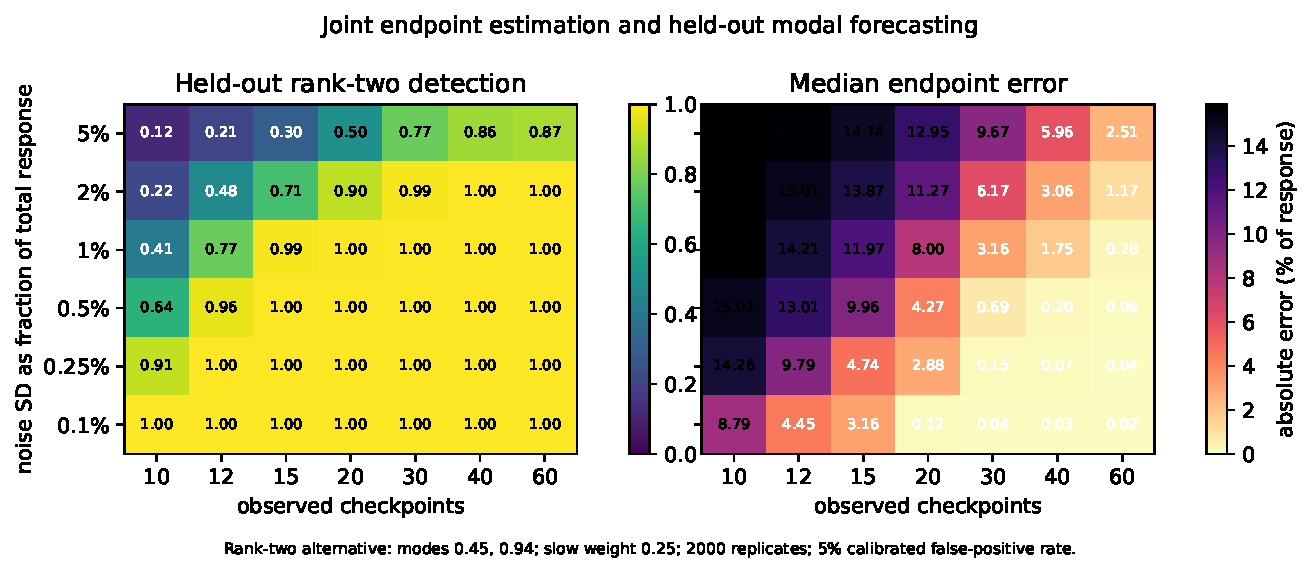
\includegraphics[width=0.96\textwidth]{figures/fig3_asymptote_forecast.pdf}
\caption{\textbf{Detection is easier than endpoint recovery.}
Rank-one and rank-two models jointly estimate the asymptote from the training
prefix and are scored on the held-out tail.  The left panel gives power to
prefer rank two under the alternative \eqref{eq:power-alternative}; the right
gives the median absolute rank-two endpoint error as a percentage of the total
response.  Each condition uses $2{,}000$ calibration, test-null, and
alternative replicates.  High model-selection power can occur while endpoint
estimation remains poor.}
\label{fig:asymptote-forecast}
\end{figure*}

The minimum tested counts attaining $0.8$ power are $10,10,12,15,20,$ and
$40$ checkpoints at noise levels $0.1\%,0.25\%,0.5\%,1\%,2\%,$ and $5\%$ of
the total response, respectively.  These are detection thresholds, not
parameter-recovery thresholds.  At $1\%$ noise, for example, power is already
$0.996$ at twenty checkpoints, yet the median endpoint error is $8.00\%$ and
both modes are recovered within $0.02$ in only $0.262$ of simulations.  At
sixty checkpoints those figures improve to $0.28\%$ and $0.901$.  Thus a
forecast failure can support ``one exponential is inadequate'' while the
ultimate endpoint and a mechanistic two-mode interpretation remain
nonidentifiable.

\section{Empirical Stress Tests}

The synthetic studies establish what the diagnostics can recover under known
conditions.  We now ask what the same hierarchy of tests says about available
self-improvement trajectories, beginning with the published evidence and then
moving to a controlled reproduction and broader forecast baselines.

\subsection{Published trajectories}

Sun et al.\ validate their law with separate exponential fits to solver
uncertainty, verifier uncertainty, and their gap over ten self-improvement
epochs, reporting $R^2>0.9$ \cite{sun2026}.  The public arXiv source contains
the vector figures but no numerical trajectories, code, or seed-level data.
We therefore performed a qualified artifact-level audit of the main Phi-4
training figure.  Its four panels each preserve twenty vector scatter points
at half-epoch spacing for all three observables, giving twelve trajectories
and $240$ figure-derived values.

For each trajectory, we fit \eqref{eq:unknown-rank-one} and
\eqref{eq:unknown-rank-two} on the first fifteen checkpoints and forecast the
last five.  A $2{,}000$-replicate parametric bootstrap calibrates $D$ under a
fitted rank-one null with independent Gaussian residuals.  Rank two has lower
held-out MSE on ten of twelve curves; nine reject at the uncorrected five
percent level, and seven remain after Holm--Bonferroni correction across the
twelve tests.  The corrected rejections comprise the Math/QE solver curve and
all solver, verifier, and gap curves in both TF panels.

The kernel reduction supplies a stronger check than twelve separate fits: the
coupled constant-coefficient law predicts one shared mode for solver,
verifier, and gap within a panel.  After equal-range normalization, a common
rank-one mode has higher held-out MSE than three separate rank-one modes in all
four panels:
\begin{center}
\begin{tabular}{lcc}
\hline
Panel & MSE factor & Holm rank-two\\
\hline
Math/QE  & $4.09$  & $1/3$\\
GSM8K/QE & $18.55$ & $0/3$\\
Math/TF  & $10.06$ & $3/3$\\
GSM8K/TF & $4.32$  & $3/3$\\
\hline
\end{tabular}
\end{center}
This comparison is descriptive because the plotted gap is algebraically
related to solver and verifier and their seed-level covariance is unavailable.
More generally, vector extraction cannot distinguish true modal structure from
endpoint error, time-varying rates, aggregation across seeds, or other smooth
misspecification.  The result therefore improves the empirical question---it
identifies a concrete failure mode and a raw-data test---without yet proving a
multi-mode mechanism.

\subsection{Fresh-seed reproduction}

We also implemented a structural rather than numerical reproduction of the
inner-clock experiment in Sun et al.\ \cite{sun2026}.  The same
Qwen2.5-0.5B-Instruct model acts as solver and True/False self-verifier.  For
each prompt it samples three candidates, filters at verifier probability
$0.5$, selects the qualifying candidate of smallest length-normalized NLL, and
uses sixteen fixed selections as pseudo-labels for rank-16 LoRA SFT.  The run
uses ten epochs, learning rate $10^{-5}$, and weight decay $0.01$.  Eight fixed
held-out arithmetic prompts are evaluated before training and twice per epoch,
giving twenty-one checkpoints.  Three declared fresh seeds change the
synthetic task sample and all sampling randomness.  This scale fits a 4 GB GTX
1650; it replaces the published 3--8B models, $N=16$, longer generations,
benchmark tasks, and A800 hardware.  A preliminary GSM8K calibration produced
no correct candidate among thirty-two samples, motivating the controlled task.

For each seed we fit signed rank-one and rank-two residual laws on the first
fifteen checkpoints and forecast the final six.  We add a last-value
persistence forecast: a richer exponential is not useful evidence if it merely
beats a poorer exponential.  The table reports pseudo-label accuracy, initial
and final solver/verifier accuracy, initial and final per-token gap, the number
of six observables on which rank two wins, and the number on which the better
modal forecast beats persistence.
\begin{center}
\scriptsize
\setlength{\tabcolsep}{3pt}
\begin{tabular}{rcccccc}
\hline
Seed & PL & $A_s$ & $A_v$ & $\bar G$ & R2 & M/P\\
\hline
20260718 & $.625$ & $.50\!\to\!.875$ & $.875\!\to\!.75$ & $.241\!\to\!-.015$ & $4/6$ & $1/6$\\
20260719 & $.625$ & $.50\!\to\!.50$ & $.625\!\to\!.625$ & $.054\!\to\!.041$ & $4/6$ & $2/6$\\
20260720 & $.625$ & $.75\!\to\!.75$ & $.875\!\to\!.875$ & $.058\!\to\!.029$ & $1/6$ & $2/6$\\
\hline
\end{tabular}
\end{center}

The per-token gap narrows in all three seeds, reproducing qualitative gap
closure, but accuracy improvement occurs only in the first.  Rank two wins
nine of eighteen series--seed forecasts, exactly half; the better modal model
beats persistence in only five.  The per-token gap is the only observable
family for which a modal model beats persistence in two seeds, and its
preferred order is not stable.  The stronger shared-mode check is also mixed.
For total NLL, shared-rank-one/separate-rank-one MSE factors are
$0.94,0.96,0.83$; for per-token NLL they are $1.00,0.73,1.44$.  The fitted
shared per-token modes $0.70,0.60,0.995$ are not a replicated system constant.

Finally, total NLL can tell a different story from per-token NLL because the
selection rule normalizes for length while the paper's uncertainty definition
does not.  Correct selected responses are often longer than single solver
samples, reversing the sign of the total-NLL gap.  Response length and both
uncertainty conventions should therefore be logged.  Overall, this experiment
reproduces gap closure but verifies neither a stable single exponential nor a
replicated second mode.  Its small evaluation panel and discrete decoding
transitions make it a falsifiable pilot, not a replacement for the published
scale.

\subsection{Rolling forecast baselines}

To test whether the modal comparison is specific and split-robust, we forecast
from five prefixes containing $50,60,70,75,$ and $80$ percent of each curve.
The candidate models are persistence, a training-only cross-validated local
linear smoother, power-law relaxation
$Y(t)=Y_\infty+c(t+\tau)^{-p}$, and signed rank-one and rank-two residuals.
The resulting winner counts are
\begin{center}
\small
\setlength{\tabcolsep}{4pt}
\begin{tabular}{lrrrrrr}
\hline
Source & Cases & Persist. & Local & Power & R1 & R2\\
\hline
Published    & $60$ & $0$  & $4$  & $27$ & $13$ & $16$\\
Reproduction & $90$ & $52$ & $10$ & $13$ & $8$  & $7$\\
\hline
\end{tabular}
\end{center}
On the published curves, at least one modal forecast beats persistence in all
sixty cases, confirming a smooth trend, but power law beats both modal models
in thirty.  No curve has one winner at all five boundaries; mean winner
consensus is $0.53$.  The earlier rank-two advantage therefore rejects a rigid
rank-one exponential without specifically identifying a second exponential
mode.  On the reproduction, the better modal model beats persistence in only
$27/90$ cases, persistence is the consensus winner for fifteen of eighteen
trajectories, and only two trajectories keep one winner across all splits.

A fixed-seed synthetic calibration uses 200 heterogeneous rank-one and 200
rank-two curves with twenty-one checkpoints and one-percent response-scale
noise.  Naively choosing the lower modal forecast MSE is correct only $0.651$
of the time and is biased toward rank two.  Calibrating the log MSE ratio at a
five-percent rank-one false-positive rate gives rank-two detection power from
$0.43$ to $0.625$ across the five splits.  Hence forecast improvement can
detect misspecification without reliably classifying modal order at this
resolution.

\subsection{Endpoint-free inverse audit}

We also apply an endpoint-free inverse diagnostic to first differences.  For
a candidate order $R$, we calibrate the squared Hankel energy beyond rank $R$
on 400 matched synthetic nulls, then recover poles with a truncated matrix
pencil.  At one-percent noise the selector chooses the correct rank-two order
in only $1.15\%$ of heterogeneous rolling cases, and even when supplied the
true order the 21-checkpoint pencil recovers both poles within $0.05$ in only
$12.5\%$.  Acceptance of rank one on all sixty published cases is therefore
non-informative.  Conditional one-pole summaries are nevertheless stable: the
median gap, solver, and verifier poles are $0.740,0.790,0.889$, respectively,
with that ordering and pairwise nonoverlapping 10th--90th percentile
perturbation intervals in all four panels.  This supplies a direct failure of
the exact shared-single-mode restriction without identifying a replacement
mode count.  On the reproduction, most cases have high numerical Hankel rank
but no stable poles, consistent with discrete jumps rather than many physical
modes.

\subsection{Global, local, and dense-start dynamics}

The first local-versus-global audit compares a shared rank-one response, a
shared rank-two response, and a continuous two-phase exponential with broader
power-law, local-linear, and persistence baselines.  On the four published
panels, shared rank two wins all $20$ structural rolling comparisons and the
two-phase model wins none against it.  Once the broader baselines are included,
separate power laws win $12$ cases, shared rank two wins $6$, separate rank one
wins $1$, and local linear wins $1$.  All $56$ published local-rate windows
fall in $(0,1)$, but their panel medians range from $0.751$ to $0.843$ with no
consistent early-to-late shift.  The fitted change point drifts with the
training prefix.  The published curves therefore look like smooth
multiscale or nonmodal relaxation, not a stable shared phase transition.

The reproduction has the opposite shape.  Shared two phase wins $11/15$
structural comparisons, with prefix-stable fitted change points at epochs
$1.0$, $1.5$, and $3.5$ for the three seeds; two of those fits use an extreme
$0.995\to0.05$ rate change.  Those fits describe delayed jumps into plateaus
more naturally than smooth startup exponentials.  Matched synthetic controls
select true two-phase dynamics only $51\%$ of the time at this checkpoint
horizon.  Thus the apparent local law is a useful measurement hypothesis, not
an identified mechanism.

To resolve that ambiguity, seed $20260719$ was rerun with evaluation after
every optimizer update through epoch $4$ (quarter-epoch spacing), followed by
the original half-epoch schedule.  The $21$ shared checkpoints agree exactly
with the original trajectory across all logged metrics, validating that the
dense measurements did not change training.  The added checkpoints localize
the largest early event to one update, from epoch $1.25$ to $1.5$: solver total
uncertainty falls from $10.416$ to $2.394$ while mean solver response length
falls from $14.375$ to $6.875$ tokens; solver accuracy falls from $0.50$ to
$0.375$, and verifier accuracy falls from $0.75$ to $0.625$.  Solver
per-token uncertainty decreases only from $0.379$ to $0.333$, while verifier
per-token uncertainty increases from $0.327$ to $0.410$.  A later verifier
transition from epoch $3.0$ to $3.25$ similarly coincides with a length increase
from $14.125$ to $18.25$ tokens and a verifier-accuracy decrease.  These are
behavioral and measurement transitions, not clean evidence of a capability
takeoff.  They also show why a general kernel remains useful when a finite
modal law fails: a concentrated or signed response can be measured without
pretending that it is a sum of stable exponentials.

\begin{figure*}[t]
\centering
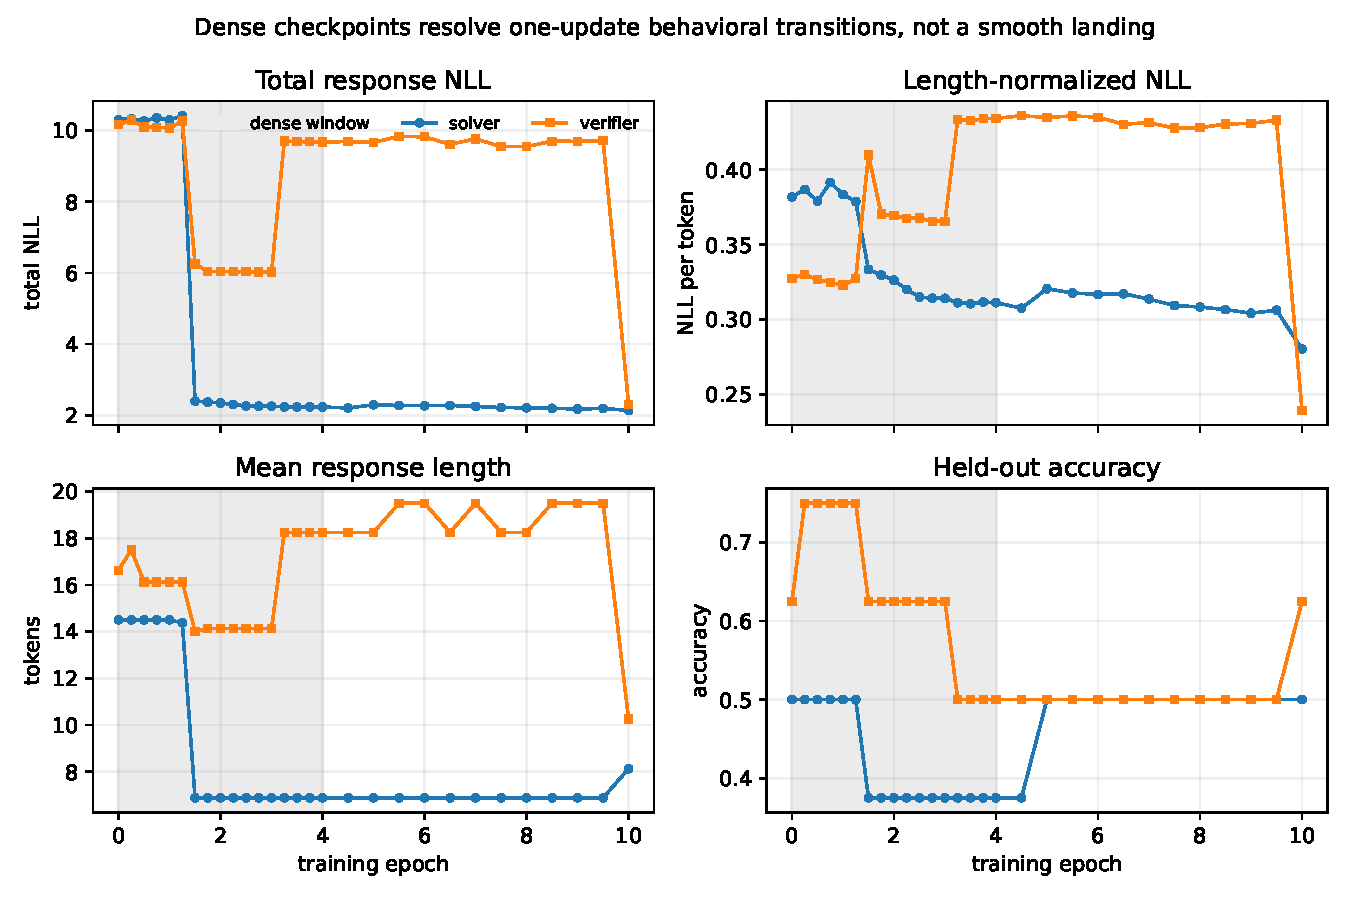
\includegraphics[width=0.94\textwidth]{figures/fig7_dense_start_audit.pdf}
\caption{\textbf{Dense-start audit for seed 20260719.} Quarter-epoch
measurements through epoch $4$ (shaded) resolve one-update transitions in total
and per-token uncertainty, response length, and accuracy.  The sharp changes
are coupled to decoding behavior and do not form a smooth exponential landing.}
\label{fig:dense-start}
\end{figure*}

\section{Experimental Implications}

The immediate experiment is a joint null test, not an unconstrained search for
complexity.  For each model--task--verifier trajectory family:
\begin{enumerate}
 \item estimate or profile over plausible asymptotes;
 \item fit one shared $\lambda$ to normalized $U_s,U_v,G$ trajectories;
 \item test kernel-ratio and Hankel-minor residuals;
 \item compare against regularized finite-modal, diffuse-spectrum, phase-changing,
 and nonparametric alternatives;
 \item evaluate by held-out checkpoints and stability across seeds.
\end{enumerate}
The synthetic studies separate two design targets.  Roughly fifteen
checkpoints can detect held-out rank-one failure for this alternative at one
percent response-scale noise, but endpoint and mode estimation require closer
to forty--sixty.  Kernel-Hankel detection is more demanding because
differencing attenuates slow modes and amplifies observation noise.  These are
conditional floors, not general prescriptions: the required count rises as
the slow-mode weight or modal separation shrinks.  In practice both residual
and kernel analyses should be reported, with asymptote sensitivity for the
former and noise-aware window selection for the latter.  Raw data should retain
paired seed-level solver, verifier, and gap measurements so that the shared-mode
null can be tested with the correct covariance.
If the available checkpoint count cannot distinguish one mode from two in a
matched synthetic study, the correct conclusion is nonidentifiability at the
available resolution, not evidence for rank one.

The resulting narrative is deliberately narrower than a general theory of
self-improvement.  The standard solver--verifier law supplies a useful null;
the takeoff-kernel reduction states exactly what that null predicts; and finite
modal, diffuse-spectrum, and time-local models supply controlled alternatives
when it fails.  Current evidence is strong enough to question one exact global
shared exponential rate, but not strong enough to name a discrete mode count,
to assert a universal local exponential, or to separate causal sources from
their aggregate response.  Better checkpoint density, independent observables,
paired seed-level trajectories, and explicit asymptote and response-length
sensitivity are the next research requirements.

\begin{thebibliography}{9}\footnotesize

\bibitem{huang2025}
A.~Huang, A.~Block, D.~J. Foster, et al.
\newblock Self-improvement in language models: The sharpening mechanism.
\newblock \emph{ICLR}, 2025.
\href{https://arxiv.org/abs/2412.01951}{arXiv:2412.01951}.

\bibitem{song2025}
Y.~Song, H.~Zhang, C.~Eisenach, S.~Kakade, D.~Foster, and U.~Ghai.
\newblock Mind the gap: Examining the self-improvement capabilities of large
language models.
\newblock \emph{ICLR}, 2025.
\href{https://arxiv.org/abs/2412.02674}{arXiv:2412.02674}.

\bibitem{sun2026}
Y.~Sun, Y.~Liang, Z.~Zhang, X.~Liu, and J.~Teng.
\newblock Theoretical modeling of large language model self-improvement
training dynamics through solver--verifier gap.
\newblock \emph{ICLR}, 2026.
\href{https://arxiv.org/abs/2507.00075}{arXiv:2507.00075}.

\end{thebibliography}

\end{document}
